\chapter{Introduction}
\label{ch:introduction}

Robotic manipulation of objects is an increasing field of research which has struggled researches from many years ago. In several industries environments robots can be easily programmed considering some standard objects, i.e. the manipulation is always the same and known, and usually robot operations avoid to deal in cluttered scene, for instance through a conveyor belt the objects are singulated from the others ones. In order to move the robots outside industries and bring them to home of people they need to be equipped with a particular intelligence and skills that are still at a first stage.
In this thesis we are going to investigate a simple approach that tries to replicate the human reasoning step during the manipulation of objects of table clearing task. The main objective is trying also to manipulate the objects in a human style, that is paying attention that during the manipulation the collision between objects is avoid as much as possible. This is a behaviour that all we do, of course with fragile objects, but also with objects that have no problem regarding collisions.  

Next, in this chapter a brief introduction of the problem and the approach used is commented, and the experimental set up as well since it will be useful to understand some techniques and choice for the algorithm. 

\section{Problem Approach}
In this section the approach to resolve the planning problem is described. All the strategy is inspired to a human like solution. A human to resolve such a task would use three main actions: grasp an object with one hand or both, when it is not possible to grasp an object because other object imped the human to put the hands in the proper way to grasp a desired object he/she has to interact with the objects in order to achieve a configuration of the objects that can be suitable to grasp an object, and this is achieved through pushing or dragging actions. Dragging an object is a very complex action which will need the robot to lay the end effector on the top of an object and make enough pressure on the contact in order that the friction between the table and the object is minor than the friction between the object and the robot's end effector. This is a very hard action which would imply an implementation of a reliable controller, because the goal is not only to move the object but also not to ruin it.  

For these considerations the main actions the robot has to use in order to interact with the objects are:
\begin{itemize}
\item Grasping
\item Pushing
\end{itemize}
Grasping is the most important action since it lets to take an object from the pile of objects and drop it somewhere, for example in a bin, clearing in this way the table. There exist different works facing the same task by focusing only in grasping. The pushing becomes useful considering the problem that two adjacent objects could not be grasped if they are so close such that the robot's gripper, when attempting to grasp an object is going to collide with an adjacent object, making such an object ungraspable. From this consideration is necessary the pushing action, in order to separate adjacent objects which could mutually exclude themselves to be grasped. Moreover the robot's intelligence is enhanced by a planning system which will return a sequence of actions in order to achieve the goal to clear the table.  

\section{Set Up}
In order to make the understanding of the approach used the name the set up of the environment the robot will work in is presented. 
The robot used is a Barret WAM arm, which is a 7 degree of freedom (DoF) manipulator arm shown in Figure \ref{fig:wam_1}. 

\begin{figure}[htp]
\centering
\begin{subfigure}[b]{0.45\textwidth}
\centering
\includegraphics[height=5cm]{Img/set_up/wam.jpg}
\caption{Barrett WAM arm}\label{fig:wam_1}
\end{subfigure}
\begin{subfigure}[b]{0.45\textwidth}
\centering
\includegraphics[width=5cm]{Img/set_up/Kinect.jpg}
\caption{Microsoft Kinect sensor}\label{fig:wam_1}
\end{subfigure}
\caption{Robot and vision sensor.}
\end{figure}

This robot is characterized by a low inertia of the end effector thanks to the kind of its actuators. The WAM is noteworthy because it does not use any gears for manipulating the joints, but rather a cable drive, so there are no backlash problems and it is both fast and stiff. Cable drives permit low friction and ripple-free torque transmission from the actuator to the joints. 




To manipulate the objects the manipulation skills of the robot are enhanced by a gripper designed in the IRI institute driven by Dynamixel motors. Such a gripper is depicted in Figure \ref{fig:gripper_general} from several point of views. 

\begin{figure}[htp]
\centering
\begin{subfigure}[b]{0.3\textwidth}
\centering
\includegraphics[height=3cm]{Img/set_up/gripper1.png}
%\caption{}
\end{subfigure}
\begin{subfigure}[b]{0.3\textwidth}
\centering
\includegraphics[height=3cm]{Img/set_up/gripper2.png}
%\caption{}
\end{subfigure}
\begin{subfigure}[b]{0.3\textwidth}
\centering
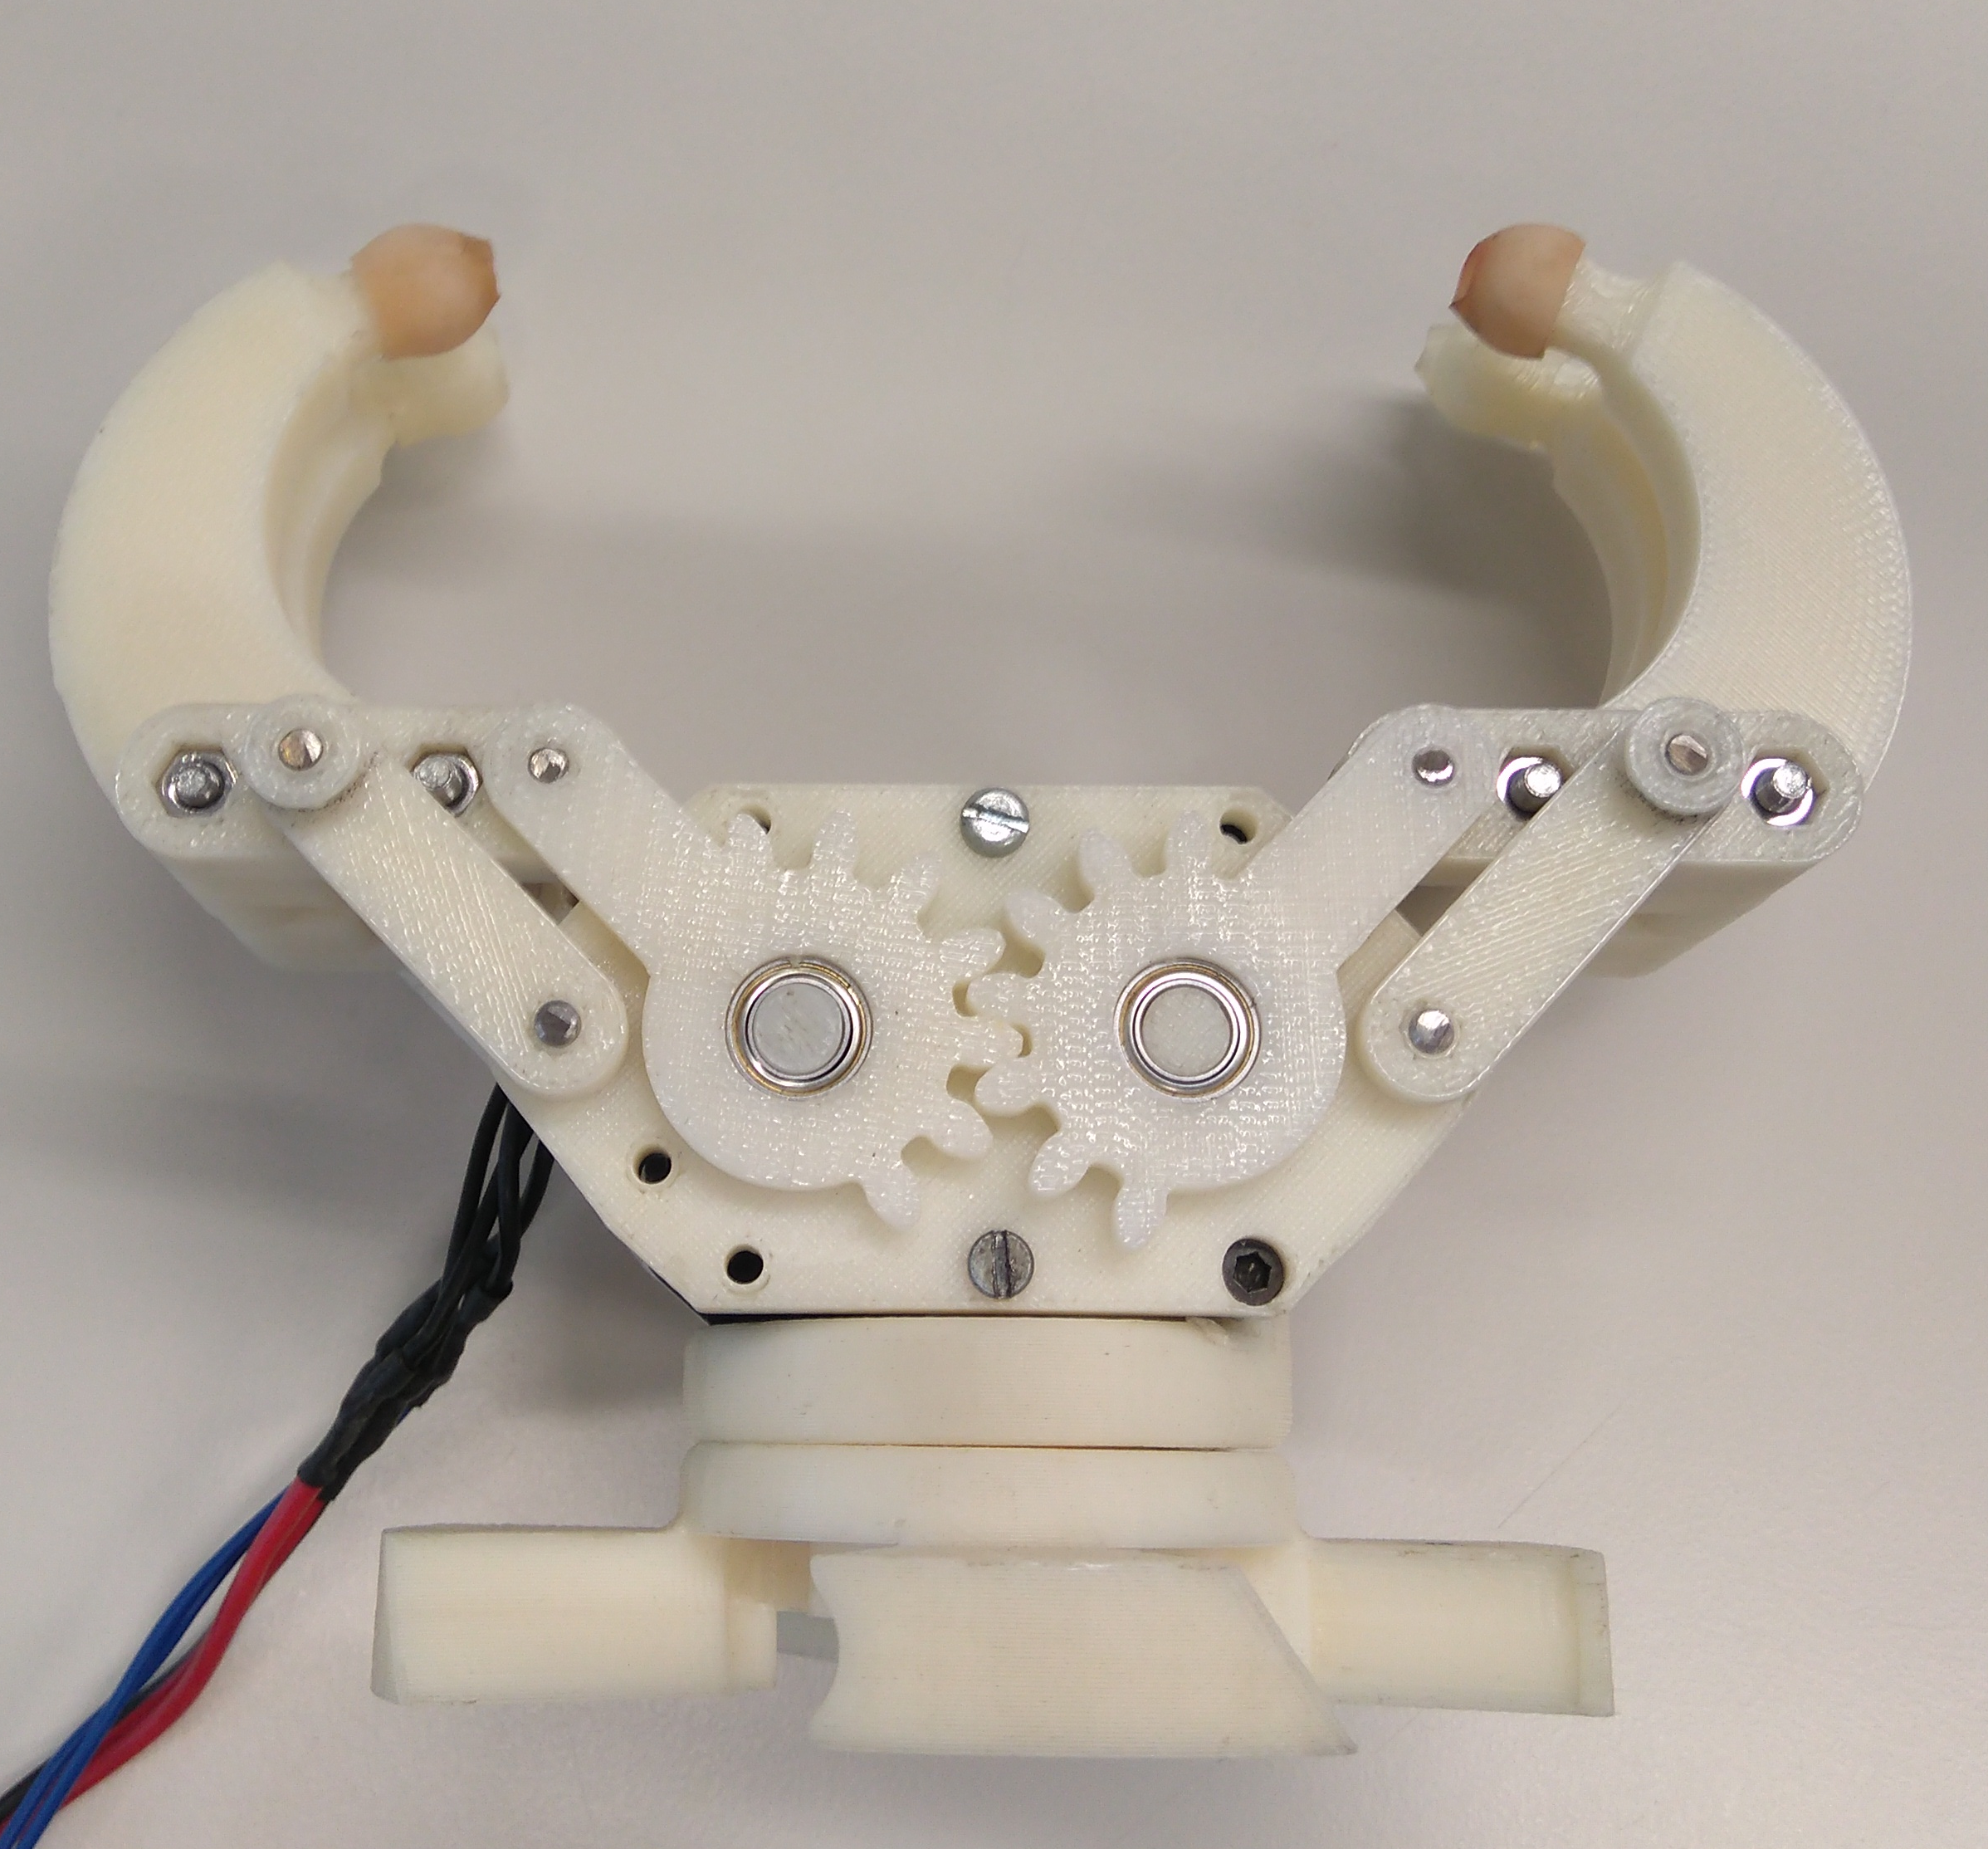
\includegraphics[width=3cm]{Img/set_up/gripper3.png}
%\caption{}
\end{subfigure}
\caption{Gripper used for the experiments}\label{fig:gripper_general}
\end{figure}

For the task planner, as the reader will see in chapters \ref{ch:task_planner} and \ref{ch:algorithm}, the model of the gripper will be an important resource 
in order to find a feasible sequence of action that can free the table.

The gripper will be modelled measuring some principal elements such as: finger's width and height, gripper's width, height and deep, and the distance between the fingers when the gripper is opened or closed. The modelling procedure is depicted in Figure \ref{fig:gripper_modelling}. The resulting model is a simple polygonal mesh which includes all the important geometric information of the gripper.

\begin{wrapfigure}{r}{6.5cm}
\caption{Gripper and WAM.}\label{fig:wam_gripper}
\includegraphics[width=5.0cm]{Img/set_up/wam_gripper.png}
\end{wrapfigure}

Such a simple model allows the collision algorithm commented in chapter \ref{ch:algorithm} to check for collision in just few millisecond. 
A more detailed and complex model would only lead as benefits a higher precision, precision that in this case is not needed, and it will slow down algorithm because the collision checking procedure would be more computationally expensive. 
The gripper will be mounted in the end effector of the robot as shown in Figure \ref{fig:wam_gripper}. 


\begin{figure}[htp]
\centering
\begin{subfigure}[t]{0.25\textwidth}
\centering
\stackunder[5pt]	{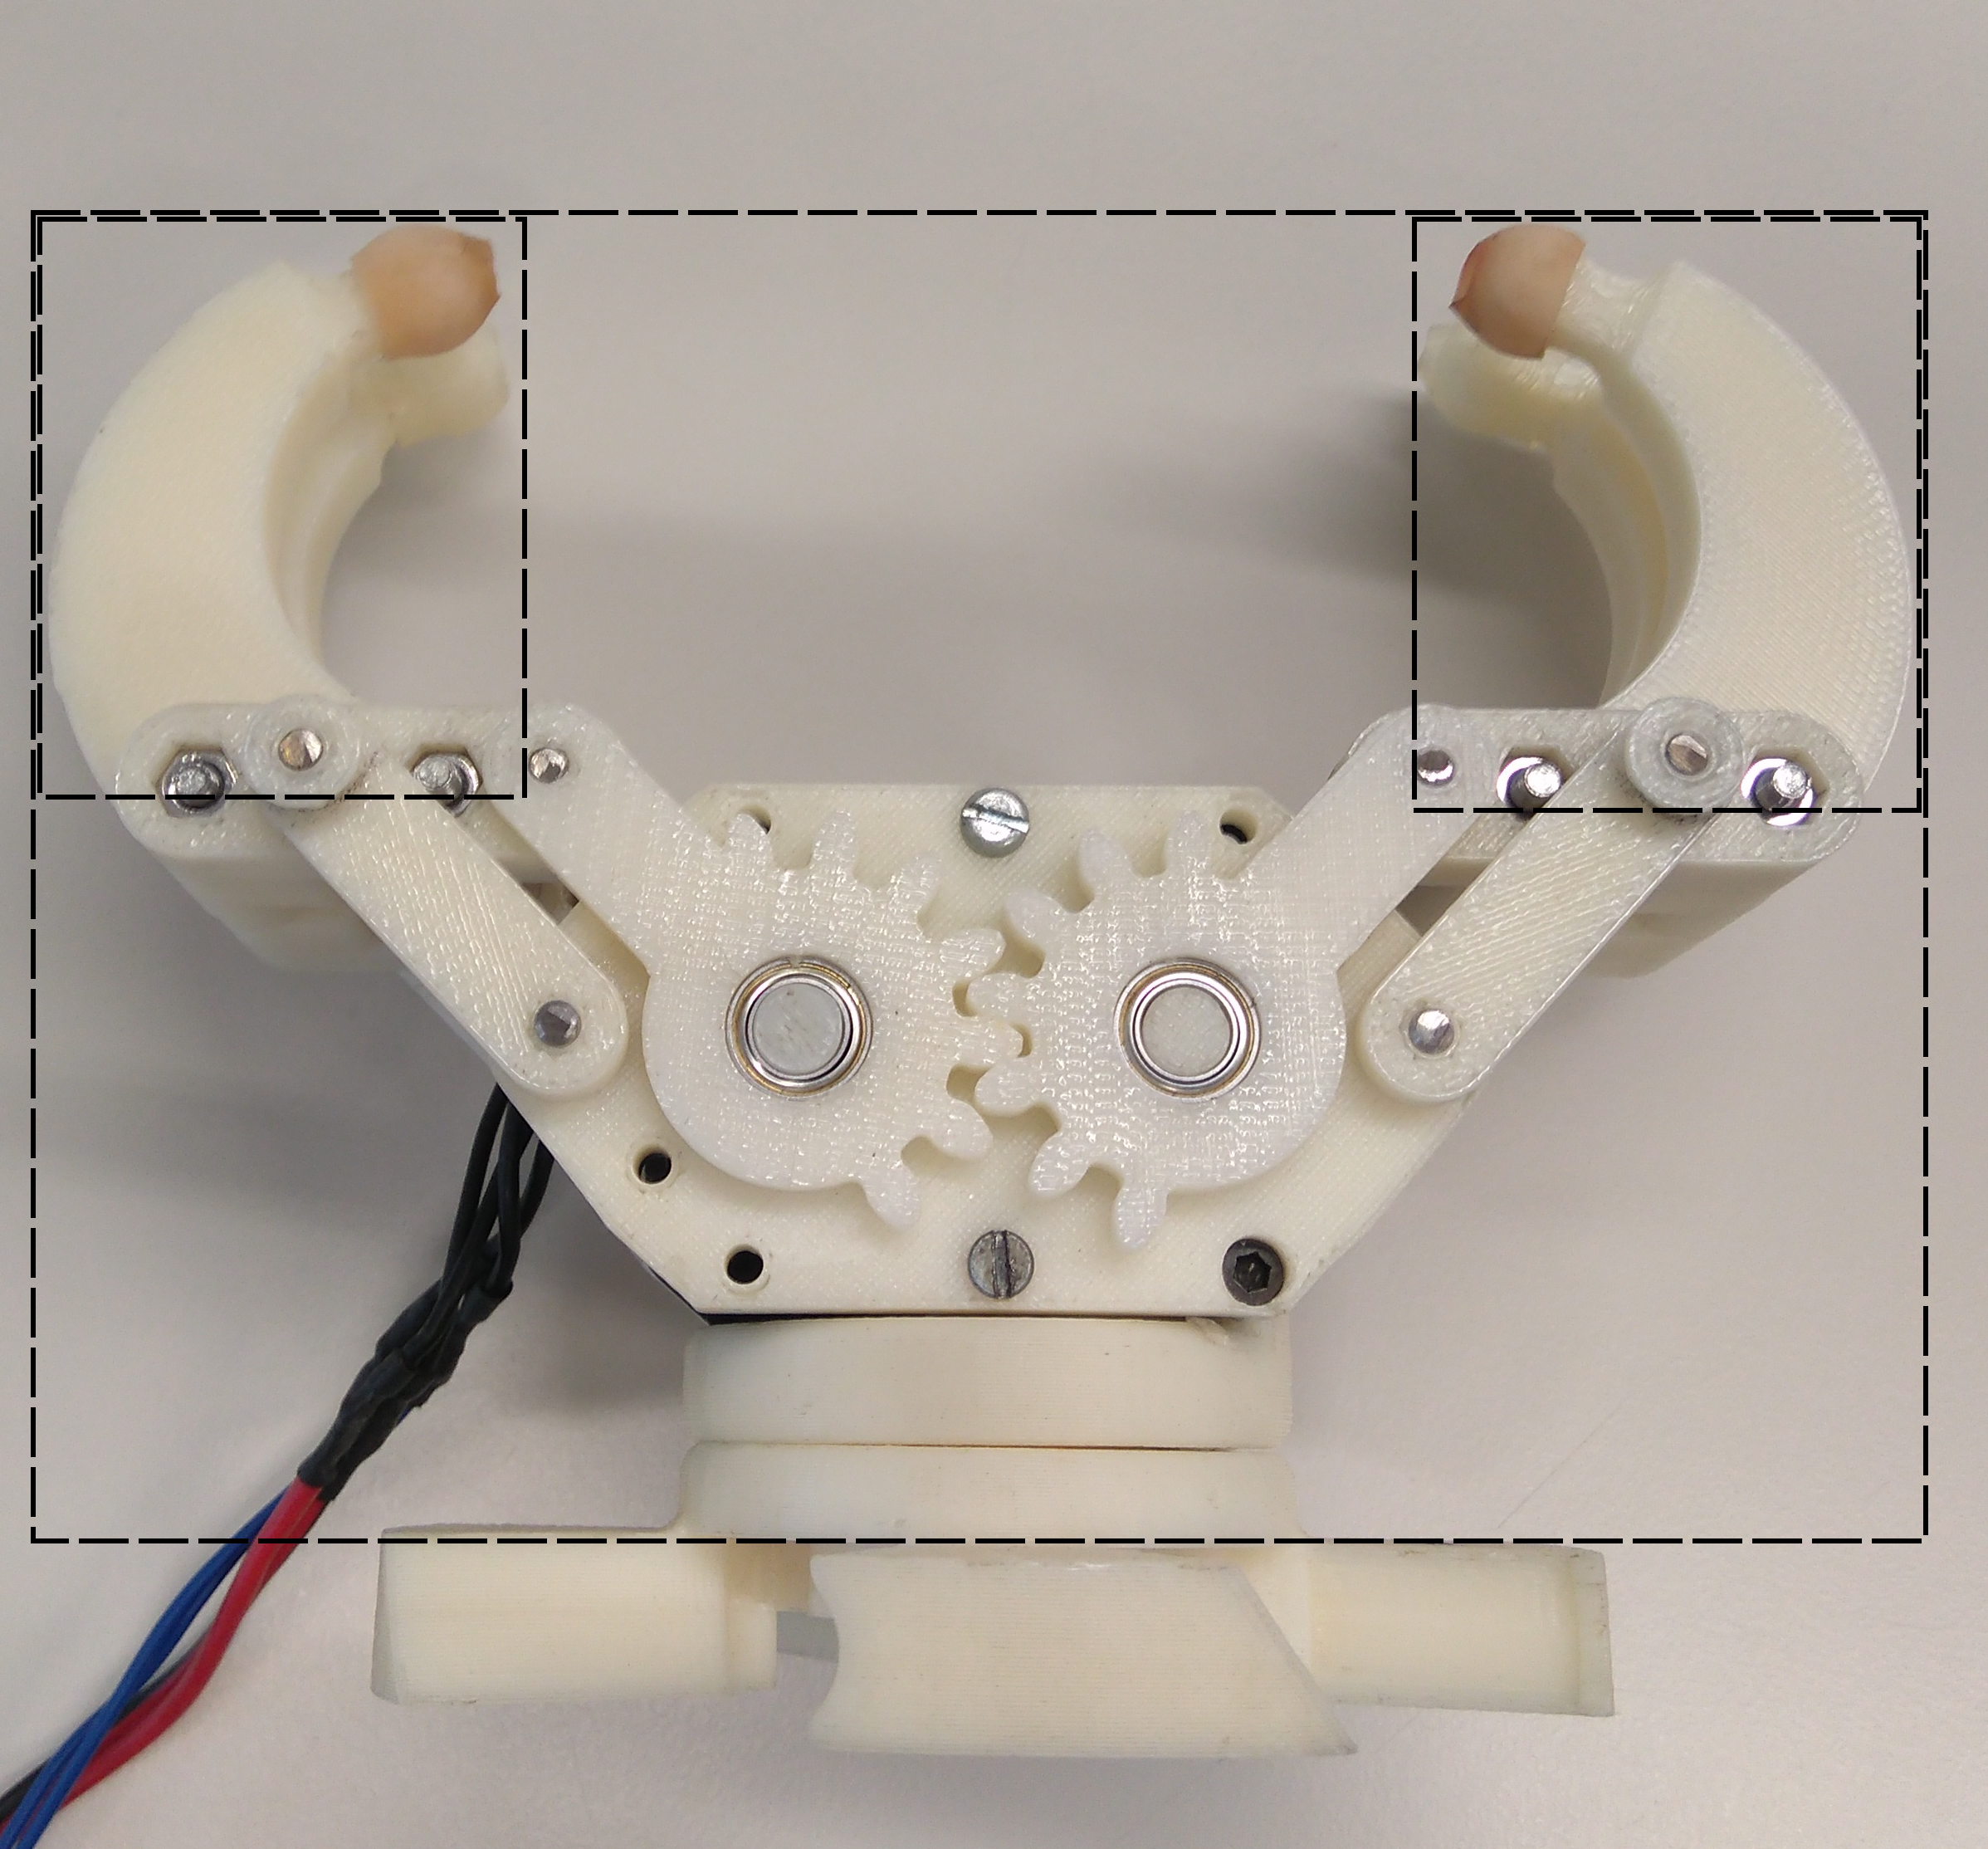
\includegraphics[height=3cm]{Img/set_up/gripper_modelling1.png}}{Elements measured}
\end{subfigure} 
\begin{subfigure}[t]{0.3\textwidth}
\centering
\stackunder[5pt]	{\includegraphics[height=3cm]{Img/set_up/gripper_open_model.png}}{Opened gripper mesh model}
\end{subfigure}
\hspace{1cm}
\begin{subfigure}[t]{0.3\textwidth}
\centering
\stackunder[5pt]	{\includegraphics[height=3cm]{Img/set_up/gripper_closed_model.png}}{Closed gripper mesh model}
%\caption{}
\end{subfigure}
\caption{Modelling of the gripper: the fingers width, fingers height, the height of the whole gripper, its width and its deep have been measured. The \textcolor{red}{red}, \textcolor{green}{green} and \textcolor{blue}{blue} axis are respectively the x, y and z axis.}\label{fig:gripper_modelling}
\end{figure}

The scenario the robot is going to work in is presented by a table, and the objects will lay on top of it. In Figure \ref{fig:setup_} the main elements of are highlighted. The WAM arm is in a fixed position with respect the table and the Kinect camera is located on top of the table pointing down. The Kinect is calibrated and the fixed transformation between the Kinect's frames and the base frame of the robot is known, so all the points measured by the Kinect can be expressed in coordinates with respect the robot's frame. An example of a cluttered scene the robot is going to deal with is depcited in Figure \ref{fig:example_scene}, and the same scene seen by the Kinect is shown in Figure \ref{fig:kinect_view}. With respect the kinect's view the robot is located at the top of the image, outside the point of view of the Kinect in order to avoid to detect the arm as an object. If the robot arm would be present in a depth image we should apply some algorithms to identify the robot arm, which could also produce important occlusions, that is hide some objects from the Kinect's view. In order to avoid all this, the depth image considered is the last one provided by the Kinect when the robot is no more in the Kinect's view (these poses are known a priori). 

\begin{figure}[htp]
\centering
\begin{subfigure}[b]{0.4\textwidth}
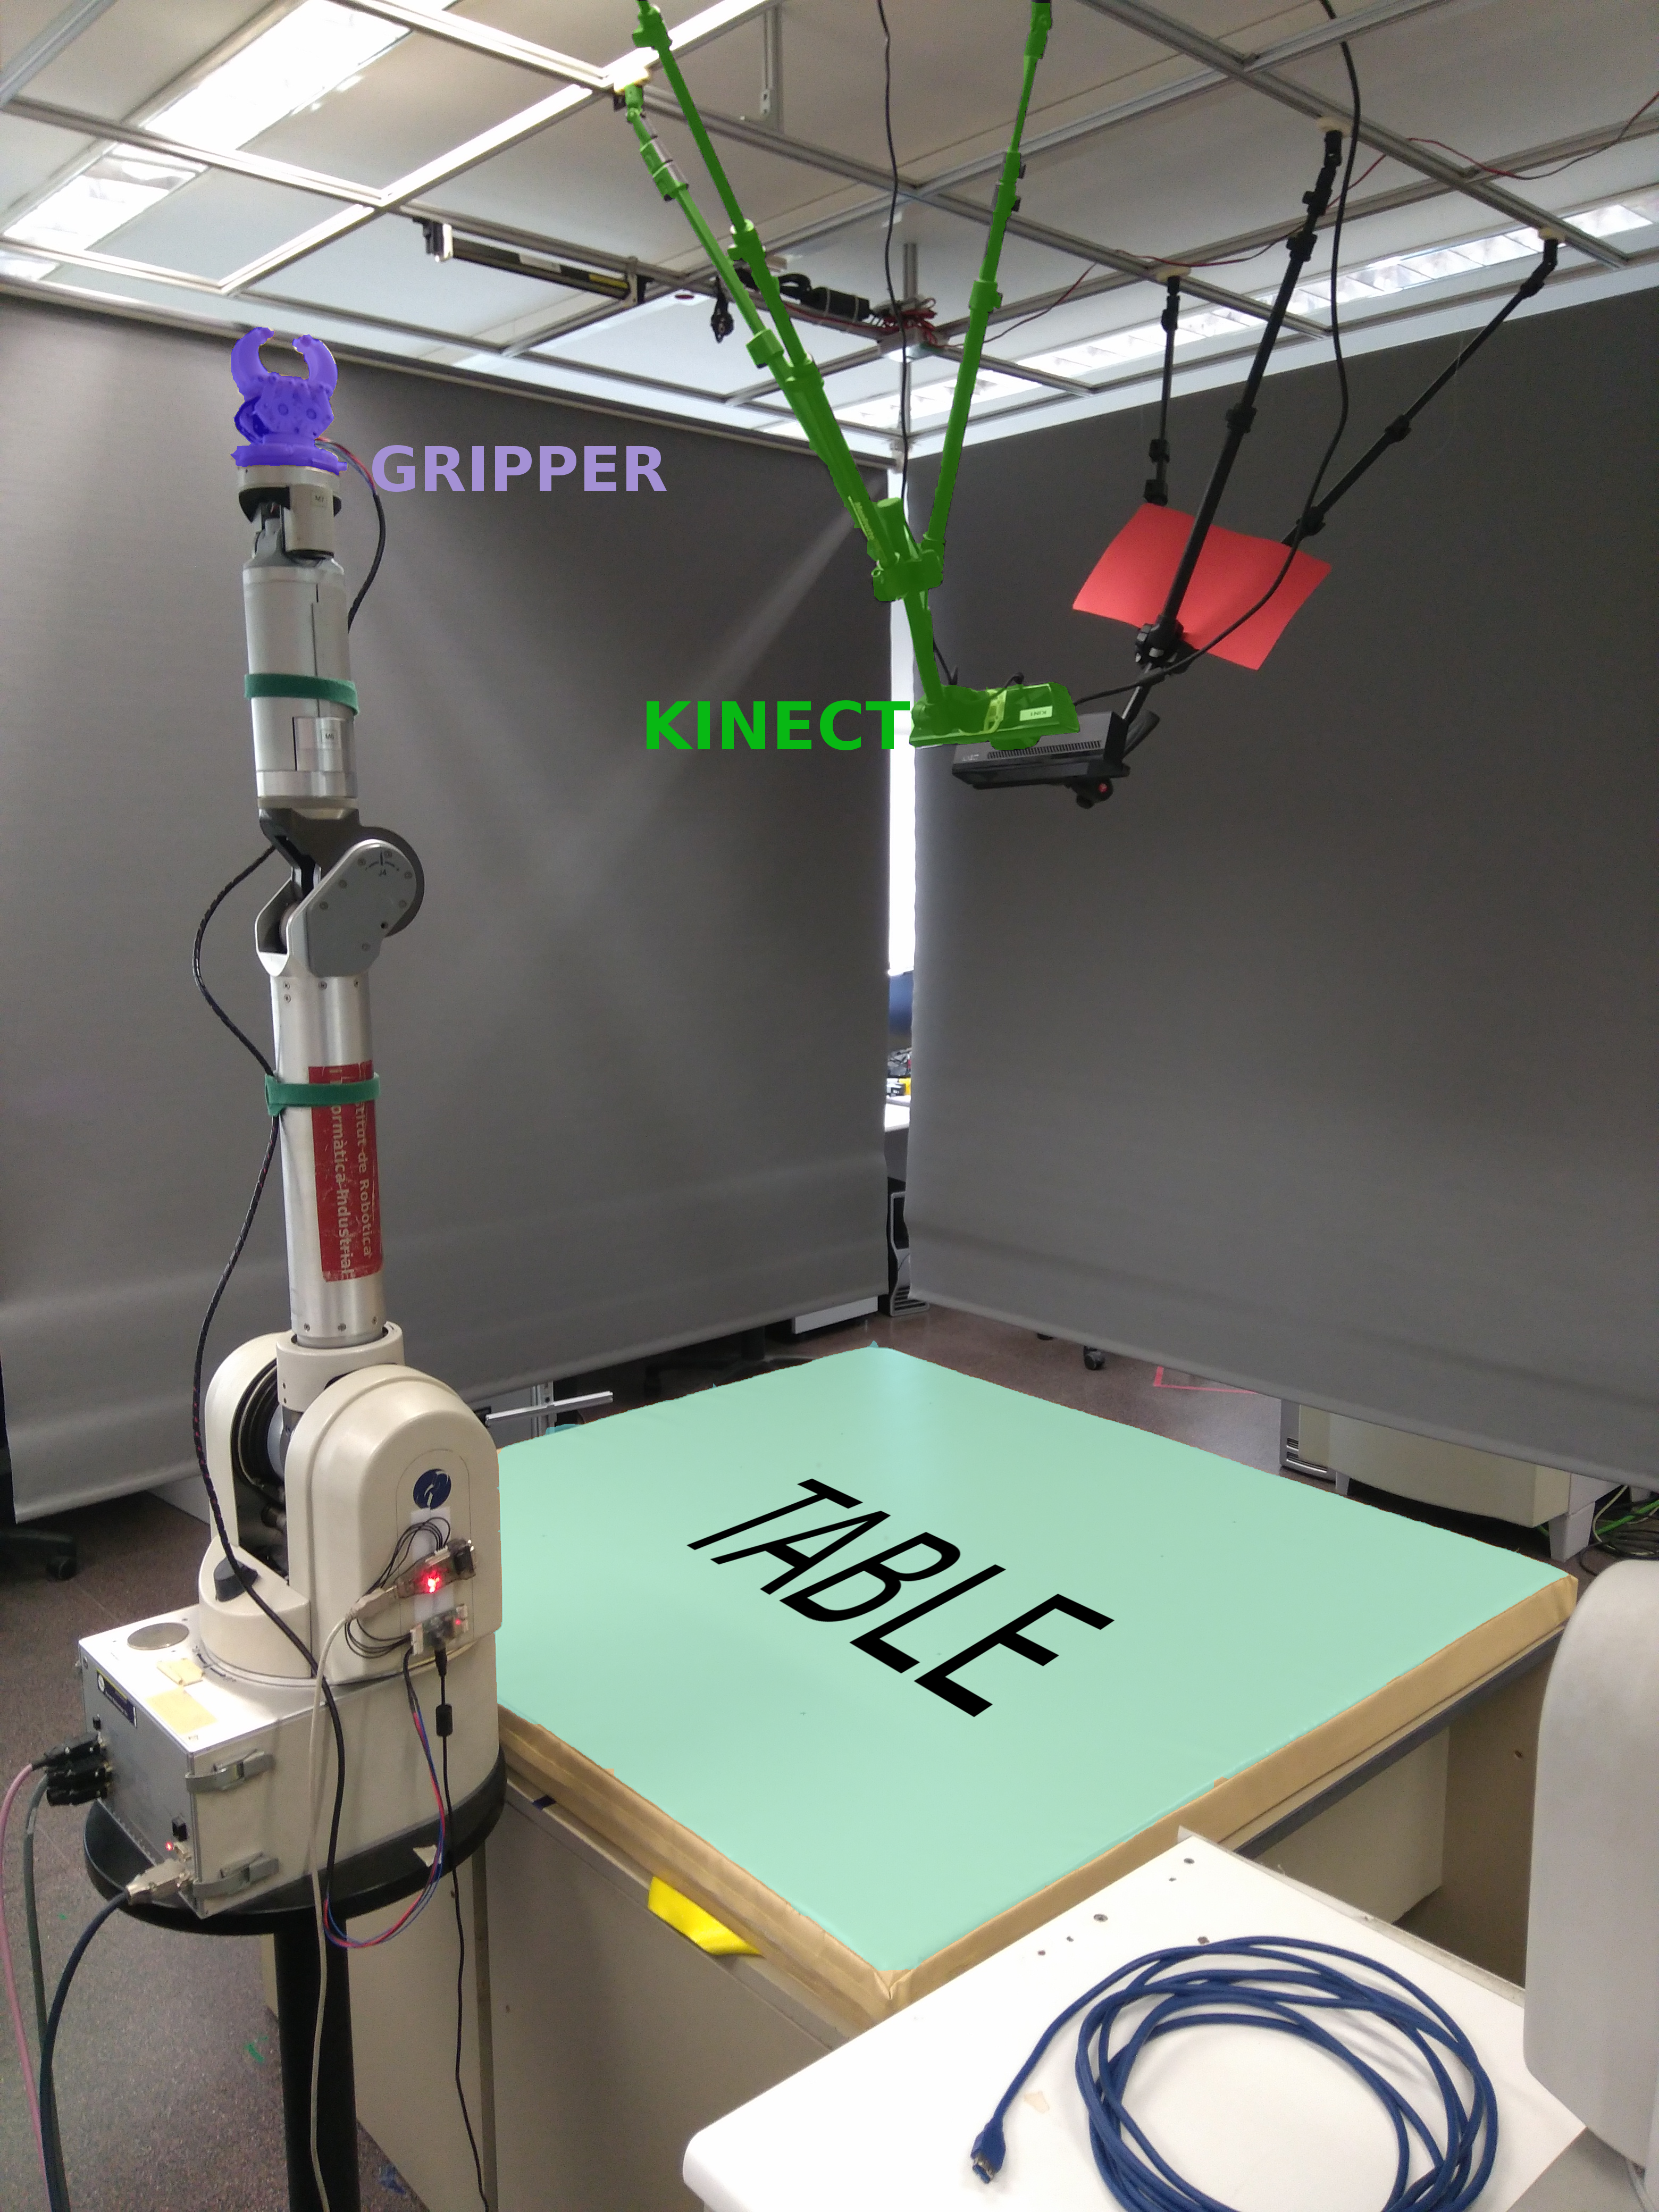
\includegraphics[height=9cm]{Img/set_up/set_up_nice.png}
\caption{Principal elements of the experimental set up.}\label{fig:setup_}
\end{subfigure}
\qquad \qquad 
\begin{subfigure}[b]{0.4\textwidth}
\centering
\includegraphics[height=4cm]{Img/set_up/example_setup.jpg}
\caption{Example of a cluttered scene the robot is going to work with.}\label{fig:example_scene}
\vspace{2ex}
\includegraphics[height=4cm]{Img/set_up/view_kinect.png}
\caption{Kinect's view.}\label{fig:kinect_view}
\end{subfigure}
\caption{Experimental set up, and example of a cluttered scene the robot is going to interact with.}
\label{fig:setup}
\end{figure}


Concerning the example of Figure \ref{fig:example_scene} it can be appreciate that the sequence of operation needed in order to clean all the table with a careful manipulation is quite complex, and due to the gripper geometry, and to the grasping poses we choose (section \ref{sec:grasping:pose}), the robot will need to grasp first the purple top object, or the white cup, then move one box in other to grasp the one of its side. All this sequence of actions will be decided by the robot.



